\documentclass{beamer}
\mode<presentation>
\usepackage{amsmath,amssymb,mathtools}
\usepackage{textcomp}
\usepackage{gensymb}
\usepackage{adjustbox}
\usepackage{subcaption}
\usepackage{enumitem}
\usepackage{multicol}
\usepackage{listings}
\usepackage{url}
\usepackage{graphicx} % <-- needed for images
\def\UrlBreaks{\do\/\do-}

\usetheme{Boadilla}
\usecolortheme{lily}
\setbeamertemplate{footline}{
  \leavevmode%
  \hbox{%
  \begin{beamercolorbox}[wd=\paperwidth,ht=2ex,dp=1ex,right]{author in head/foot}%
    \insertframenumber{} / \inserttotalframenumber\hspace*{2ex}
  \end{beamercolorbox}}%
  \vskip0pt%
}
\setbeamertemplate{navigation symbols}{}

\lstset{
  frame=single,
  breaklines=true,
  columns=fullflexible,
  basicstyle=\ttfamily\tiny   % tiny font so code fits
}

\numberwithin{equation}{section}

% ---- your macros ----
\providecommand{\nCr}[2]{\,^{#1}C_{#2}}
\providecommand{\nPr}[2]{\,^{#1}P_{#2}}
\providecommand{\mbf}{\mathbf}
\providecommand{\pr}[1]{\ensuremath{\Pr\left(#1\right)}}
\providecommand{\qfunc}[1]{\ensuremath{Q\left(#1\right)}}
\providecommand{\sbrak}[1]{\ensuremath{{}\left[#1\right]}}
\providecommand{\lsbrak}[1]{\ensuremath{{}\left[#1\right.}}
\providecommand{\rsbrak}[1]{\ensuremath{\left.#1\right]}}
\providecommand{\brak}[1]{\ensuremath{\left(#1\right)}}
\providecommand{\lbrak}[1]{\ensuremath{\left(#1\right.}}
\providecommand{\rbrak}[1]{\ensuremath{\left.#1\right)}}
\providecommand{\cbrak}[1]{\ensuremath{\left\{#1\right\}}}
\providecommand{\lcbrak}[1]{\ensuremath{\left\{#1\right.}}
\providecommand{\rcbrak}[1]{\ensuremath{\left.#1\right\}}}
\theoremstyle{remark}
\newtheorem{rem}{Remark}
\newcommand{\sgn}{\mathop{\mathrm{sgn}}}
\providecommand{\abs}[1]{\left\vert#1\right\vert}
\providecommand{\res}[1]{\Res\displaylimits_{#1}}
\providecommand{\norm}[1]{\lVert#1\rVert}
\providecommand{\mtx}[1]{\mathbf{#1}}
\providecommand{\mean}[1]{E\left[ #1 \right]}
\providecommand{\fourier}{\overset{\mathcal{F}}{ \rightleftharpoons}}
\providecommand{\system}{\overset{\mathcal{H}}{ \longleftrightarrow}}
\providecommand{\dec}[2]{\ensuremath{\overset{#1}{\underset{#2}{\gtrless}}}}
\newcommand{\myvec}[1]{\ensuremath{\begin{pmatrix}#1\end{pmatrix}}}
\let\vec\mathbf

\title{Matgeo Presentation - 8.2.31}
\author{ee25btech11063 - Vejith}

\begin{document}


\frame{\titlepage}
\begin{frame}{Question}
Find the equation of conic if ends of the major axis are \brak{\pm 3,0} and ends of the minor axis are  \brak{0,\pm 2}
\end{frame}

\begin{frame}{Solution}
    The equation of conic is represented as
\begin{align}
\vec{x}^\top\vec{V}\vec{x} + 2\vec{u}^\top\vec{x} + f = 0\\
\vec{V}=\norm{\vec{n}}^2\vec{I}-e^2\vec{n}\vec{n}^\top
\end{align}
As the major axis is along the X-axis 
\begin{align}
    \vec{n}=\vec{e_1}\\
    \implies \vec{V}=\begin{pmatrix}
        1-e^2 & 0\\
        0 & 1
    \end{pmatrix}
\end{align}
as the centre of ellipse is $\vec{c}$= $\vec{0}$
\begin{align}
    \implies \vec{u}=\vec{0}
\end{align}
let
\begin{align}
    \vec{P}=\myvec{0\\2}
\end{align}
$\vec{P}$  satisfy (1)
\end{frame}
\begin{frame}{Solution}
\begin{align}
    \vec{P}^\top\vec{V}\vec{P} + 2\vec{u}^\top\vec{P} + f = 0\\
    \brak{0\hspace{0.5cm} 2} \begin{pmatrix}
        1-e^2 & 0\\
        0 & 1
    \end{pmatrix}\myvec{0\\2} +f=0\\
     4+f=0 \\
     \implies f=-4
\end{align}
End of the ellipse $\myvec{3\\0}$ also satisfy (1)
\begin{align}
    \brak{3\hspace{0.5cm} 0} \begin{pmatrix}
        1-e^2 & 0\\
        0 & 1
    \end{pmatrix}\myvec{3\\0} +f=0\\
    \implies 9\brak{1-e^2}+f=0
\end{align}
from (10)
\end{frame}

\begin{frame}{Conclusion}
\begin{align}
    1-e^2=\frac{4}{9}\\
    \implies e^2=\frac{5}{9}\\
    \implies \vec{V}= \begin{pmatrix}
        \frac{4}{9} & 0\\
        0 & 1
    \end{pmatrix}
\end{align}
Equation of conic is 
\begin{align}
   \vec{x}^\top \begin{pmatrix}
        \frac{4}{9} & 0\\
        0 & 1
    \end{pmatrix} \vec{X}-4=0
\end{align}
\end{frame}

\begin{frame}{Plot}
    \begin{figure}
        \centering
        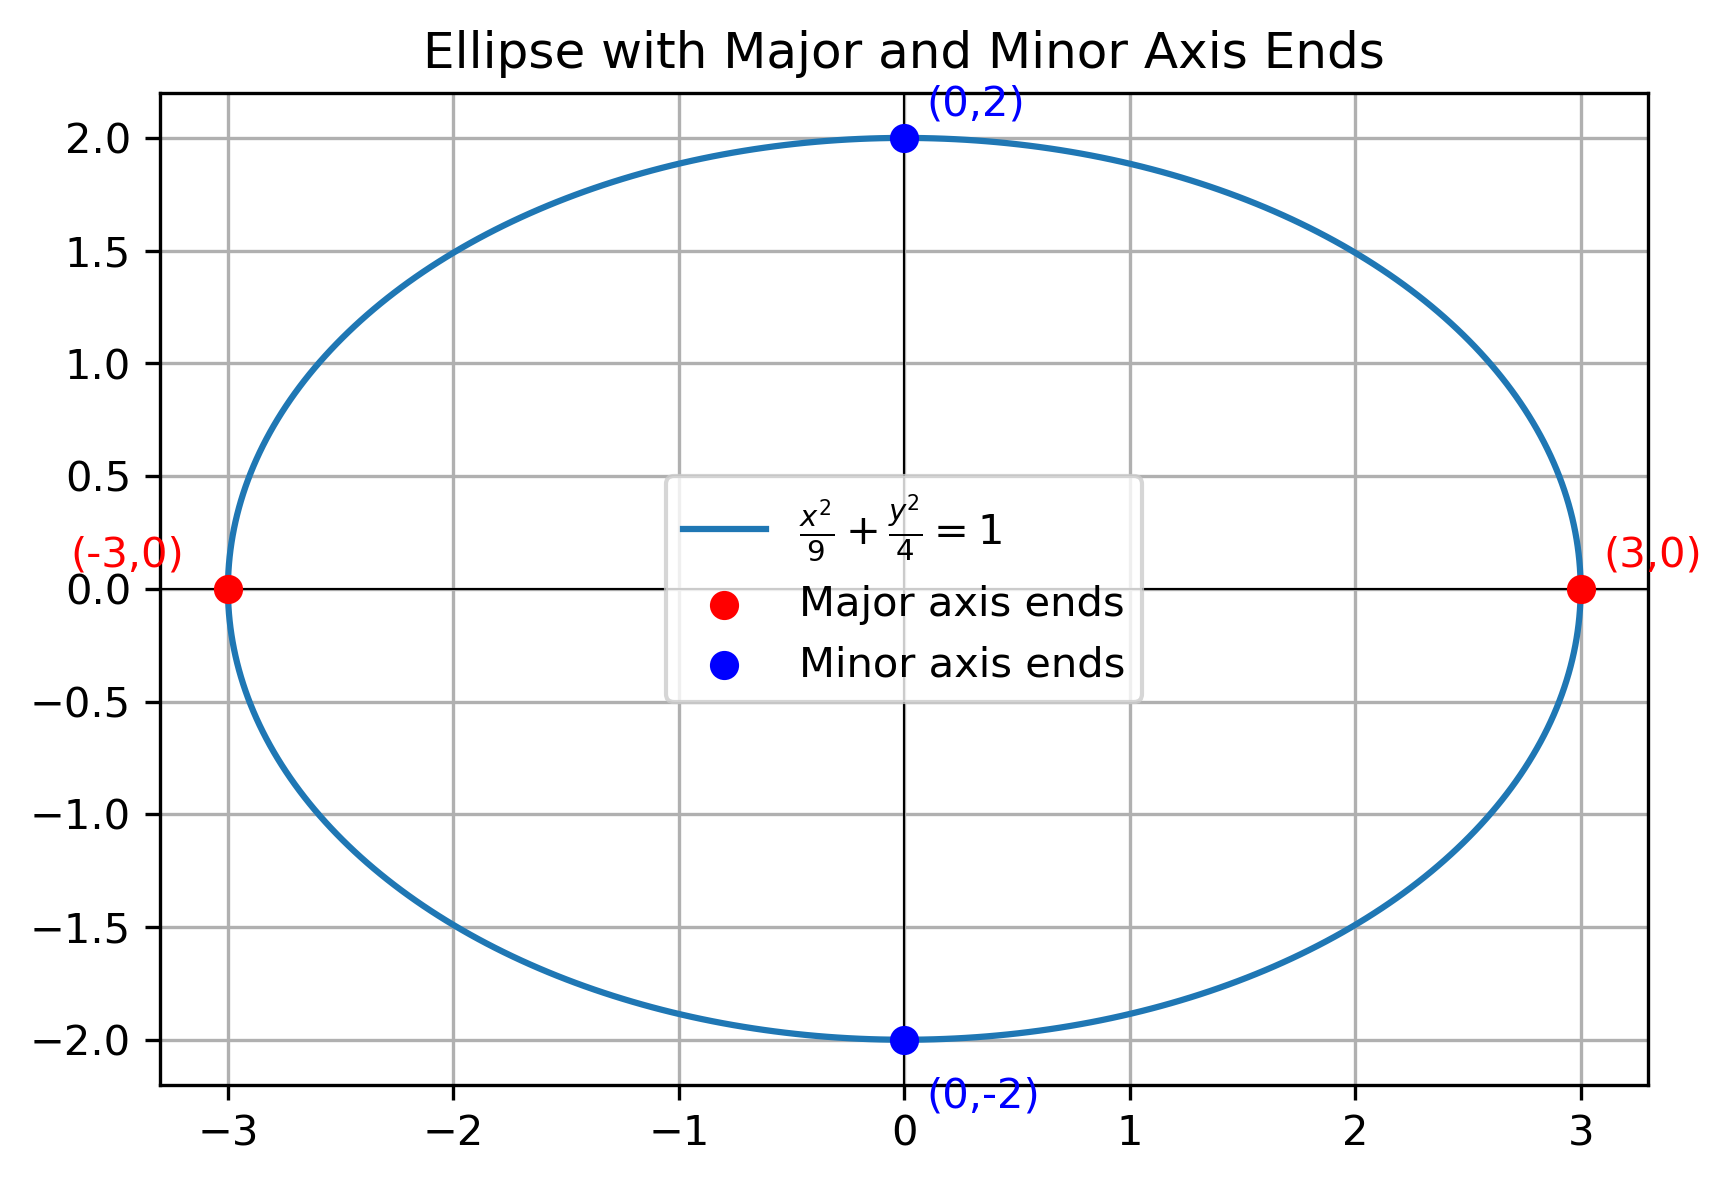
\includegraphics[width=0.8\columnwidth]{figs/01.png}
        \caption{Caption}
        \label{fig:placeholder}
    \end{figure}
\end{frame}

% --------- CODE APPENDIX ---------
\section*{Appendix: Code}

% C program
\begin{frame}[fragile]{C Code: ellipse.c}
\begin{lstlisting}[language=C]
#include <stdio.h>

int main() {
    FILE *fp;

    // Open file ellipse.dat for writing
    fp = fopen("ellipse.dat", "w");
    if (fp == NULL) {
        printf("Error opening file!\n");
        return 1;
    }

    // Write the equation of ellipse into the file
    fprintf(fp, "Equation of the ellipse:\n");
    fprintf(fp, "(x^2)/9 + (y^2)/4 = 1\n");

    // Optionally write the matrix form as well
    fprintf(fp, "\nMatrix form:\n");
    fprintf(fp, "[x y] * [[1/9  0]\n");
    fprintf(fp, " [0   1/4]] * [x y]^T = 1\n");

    fclose(fp);
    printf("Equation successfully written to ellipse.dat\n");

    return 0;
}


\end{lstlisting}
\end{frame}

\begin{frame}[fragile]{Python: plot.py}
\begin{lstlisting}[language=Python]
import numpy as np
import matplotlib.pyplot as plt

# Parameters of the ellipse
a = 3  # semi-major axis
b = 2  # semi-minor axis

# Generate theta values
theta = np.linspace(0, 2*np.pi, 400)

# Parametric equations of ellipse
x = a * np.cos(theta)
y = b * np.sin(theta)

# Plot ellipse
plt.plot(x, y, label=r"$\frac{x^2}{9}+\frac{y^2}{4}=1$")

# Mark ends of major axis (±3,0)
plt.scatter([3, -3], [0, 0], color="red", zorder=5, label="Major axis ends")

# Mark ends of minor axis (0,±2)
plt.scatter([0, 0], [2, -2], color="blue", zorder=5, label="Minor axis ends")

# Add annotations
plt.text(3.1, 0.1, "(3,0)", color="red")
plt.text(-3.7, 0.1, "(-3,0)", color="red")
plt.text(0.1, 2.1, "(0,2)", color="blue")
plt.text(0.1, -2.3, "(0,-2)", color="blue")

# Axes setup
plt.axhline(0, color="black", linewidth=0.5)
plt.axvline(0, color="black", linewidth=0.5)
plt.gca().set_aspect('equal')  # keep aspect ratio equal
\end{lstlisting}
\end{frame}

\begin{frame}[fragile]{Python: plot.py}
\begin{lstlisting}[language=Python]
plt.legend()
plt.title("Ellipse with Major and Minor Axis Ends")
plt.grid(True)
plt.savefig("ellipse.png", dpi=300, bbox_inches="tight")
plt.show()


\end{lstlisting}
\end{frame} 

\end{document}
